\section{Results}

  This section presents the results of the experimental and analytical work.
  The results of RAM model analysis are in the first subsection for reference.
  The second subsection contains the results of analysis under the VAT model.
  The results of the implementation and measurement reside in the third
  section.

  \subsection{RAM}
    This paper selected five reference algorithms, with running times well 
    studied under the RAM model. The following table presents those running
    times. These will be used later to make comparisons. Where there is a
    difference in average and worst case with Quicksort, the average case
    running time is the tested case.
    
    \begin{tabular}{ccc}
      Algorithm     & Average Case  & Worst Case   \\\hline
      BinarySearch  & $O(\log(n))$  & $O(\log(n))$ \\
      Heapsort      & $O(n\log(n))$ & $O(n\log(n))$\\
      Insertionsort & $O(n^2)$      & $O(n^2)$     \\
      Permute       & $O(n)$        & $O(n)$       \\
      Quicksort     & $O(n\log(n))$ & $O(n^2)$     \\
    \end{tabular}
    
    It is left as an excersize for the skeptical reader to look these up in any
    algorithms reference text.

  \subsection{VAT}
    The VAT model presents more of a challenge than checking a reference text.
    Jurkiewicz and Mehlorn provided analyses[5] for two of the algorithms. 
    Those results are here:
    
    \begin{tabular}{cc}
      Algorithm    & VAT Complexity\\\hline
      BinarySearch &
$O\left(\frac{r}{k}\log(\frac{2n}{P})\log(\frac{2dn}{W})\right)$ \\
      Heapsort     & $O\left(r(d+\frac{pn}{P})\right)$ \\
    \end{tabular}
    
    Where $r$ is the unit cost of translation (length/number of insertions in
    the TC). $d$ is the length of translation. $W$ represents the nodes of the
    translation tree that are in the TC. $P$ is the page size. And, $n$ is the
    input size.
  
  \subsection{Benchmarks}
    Benchmarking the algorithms on a modern computer is a key step in
    determining whether VAT or RAM more accurately models a computer for the
    purposes of algorithm analysis.
    
    BinarySearch of an integer array was the first algorithm measured.
    Reviewing the results of timing, one would see all search times as 0.000000
    seconds. The BinarySearch procedure executed too quickly, even on a 2 GiB
    array, to produce a result within the precision of the program's
    measurement.
   
    The sorting algorithms were executed on randomly generated integer arrays,
    and the permute procedure was executed on a sorted array to yield a
    randomized array of integers. The accompanying scatter plots show the
    execution times of each procedure at each size input.
   
   \begin{center}
    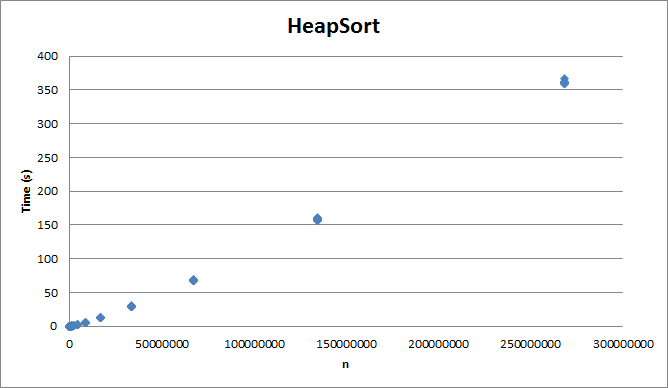
\includegraphics[width=4in]{heapsort.png}\\
    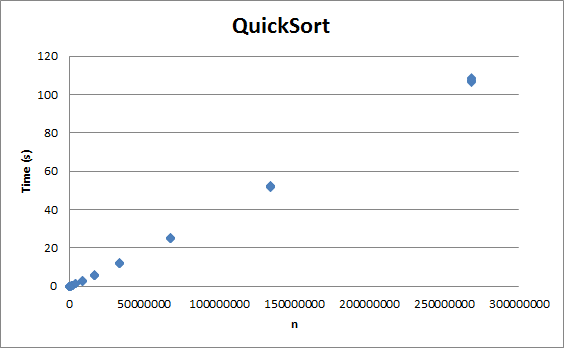
\includegraphics[width=4in]{quicksort.png}
   \end{center}
   
   The Heapsort and Quicksort times were consistent with $O(n\log(n))$
   runtimes. Heapsort has a much higher absolute running time and other
   behaviour consistent with that algorithm requiring a lengthier procedure.
   
   \begin{center}
    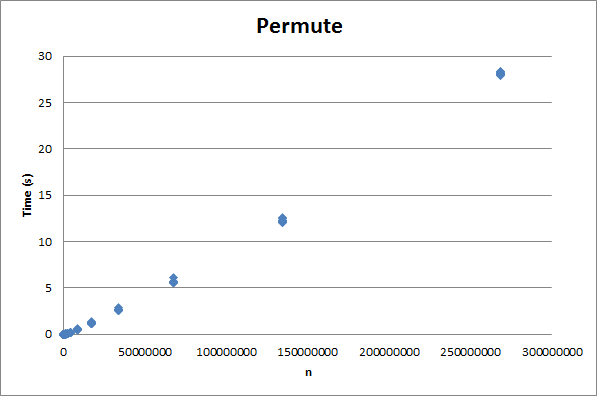
\includegraphics[width=4in]{permute.png}
   \end{center}
   
   The Permute procedure shows linear time behaviour.
   
   \begin{center}
    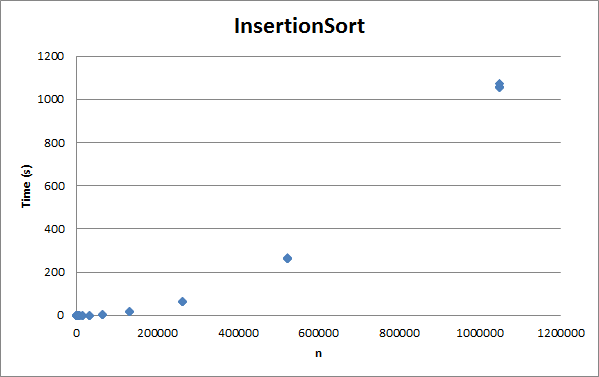
\includegraphics[width=4in]{insertionsort.png}
   \end{center}
   
   Insertionsort shows a $O(n^2)$ running time that one sees very clearly on
   the above scatterplot.